\documentclass{article}

\usepackage[preprint]{neurips_2024}

\usepackage{amsmath,amssymb}
\usepackage{booktabs}
\usepackage{graphicx}
\usepackage{xcolor}
\usepackage{url}
\usepackage{caption}
\usepackage{float}
\usepackage[hidelinks]{hyperref}

\title{Diffusion-Based Reranking for Conversational Memory Retrieval\thanks{Code available at \url{https://github.com/chainerprince/difussed_memory}}}

\author{
  Medha Ravi \And
  Otis Otieno Robert \And
  Ernest Adjetey \And
  Prince Mutegetsi
}


\begin{document}
\maketitle

\begin{abstract}
Conversational agents need to retrieve user-specific memories from large, noisy banks of facts. This project studies whether a conditional denoising diffusion model can improve top-1 memory retrieval beyond direct Sentence-BERT similarity. We embed heuristic and T5-generated queries with all-MiniLM-L6-v2, retrieve a top-$K$ candidate set with cosine similarity, and rerank candidates using a diffusion model conditioned on the query and memory-bank summary. We evaluate two diffusion strategies: prototype generation, which samples an answer embedding from the learned reverse process, and denoising-score reranking, which treats small denoising changes as evidence that a candidate lies on the conditional answer manifold. We compare against BM25 ($9.73\%$) and a MiniLM cross-encoder ($20.91\%$) as competing rerankers. On simple heuristic queries, raw SBERT reaches $17.84\%$ top-1 accuracy, while the best diffusion-only setting reaches $19.51\%$ and an ensemble reaches $20.03\%$---outperforming BM25 by a large margin and approaching the cross-encoder upper baseline. On real T5-generated queries, raw SBERT is much stronger at $51.60\%$; a real-turn-trained diffusion reranker improves to $52.40\%$ while a top-5 oracle reaches $67.60\%$. These results suggest that diffusion is a competitive reranking signal within a strong candidate set.
\end{abstract}

%% ========================================================
\section{Introduction}
%% ========================================================

Long-running dialogue systems must remember facts such as user preferences, locations, occupations, and hobbies. As conversations extend across multiple sessions, the accumulated memory bank can grow to hundreds or thousands of individual facts, making accurate retrieval increasingly challenging. A common approach is to embed the current query and all stored memory facts into a shared vector space, then retrieve the highest-scoring fact by cosine similarity~\cite{reimers2019sbert}. This paradigm is simple, fast, and benefits from the representational power of pretrained language models. However, it can fail when many memories are semantically close or when the query is underspecified, because a single dot-product score may not capture the nuanced compatibility between a conversational context and a specific fact.

Recent work on dense passage retrieval has demonstrated the effectiveness of embedding-based methods for open-domain question answering~\cite{karpukhin2020dpr}, while neural reranking models such as ColBERT~\cite{khattab2020colbert} and cross-encoder architectures~\cite{nogueira2020passage} have shown that a second-stage scoring model can substantially improve retrieval quality. Independently, denoising diffusion probabilistic models~\cite{ho2020ddpm} have emerged as powerful generative models in continuous spaces, with extensions to score-based formulations~\cite{song2021scorebased} and accelerated sampling~\cite{song2021ddim}. These models learn to reverse a gradual noising process, effectively capturing complex, multimodal distributions over continuous vectors.

We explore a diffusion-based alternative for memory retrieval that sits at the intersection of these two lines of work. Instead of directly predicting a discrete memory, the model learns a distribution over answer embeddings conditioned on the query and the memory bank. At inference time, the diffusion model is used to rerank the top-$K$ candidates returned by SBERT, rather than to generate answers from scratch. The central question is whether a generative denoising signal can recover correct facts that are already present in the top-$K$ set but not ranked first by cosine similarity.

Our contributions are as follows. First, we propose two diffusion-based reranking strategies---prototype generation and denoising-score reranking---and evaluate them on a large-scale conversational memory retrieval task derived from the Multi-Session Chat dataset~\cite{xu2022msc}. Second, we show that diffusion reranking yields statistically significant improvements on heuristic queries, with McNemar's test confirming that the reranker corrects a meaningful number of retrieval errors. Third, we demonstrate that query distribution matters: a diffusion model trained on template-style queries transfers poorly to natural T5-generated queries, but retraining on realistic dialogue turns recovers much of the benefit. Finally, we analyze top-$K$ oracle accuracy to quantify the remaining reranking headroom and identify directions for future improvement.

The remainder of this paper is organized as follows. Section~\ref{sec:related} reviews related work on retrieval, reranking, and diffusion models. Section~\ref{sec:task} describes the task and dataset. Sections~\ref{sec:baseline}--\ref{sec:reranking} present the embedding baseline and the diffusion model. Section~\ref{sec:results} reports experimental results, followed by statistical analysis in Section~\ref{sec:stats}, discussion in Section~\ref{sec:discussion}, and conclusions in Section~\ref{sec:conclusion}.

%% ========================================================
\section{Related Work}
\label{sec:related}
%% ========================================================

\textbf{Memory-augmented dialogue.}
The challenge of maintaining long-term memory across conversation sessions has been studied in the context of persona-grounded dialogue~\cite{zhang2018personalizing} and multi-session chat~\cite{xu2022msc}. In these settings, agents must track and retrieve user-specific facts such as preferences, biographical details, and opinions over conversations spanning days or weeks. Most approaches rely on explicit memory banks paired with retrieval mechanisms, though the optimal retrieval strategy remains an open question.

\textbf{Dense retrieval and reranking.}
Dense passage retrieval (DPR)~\cite{karpukhin2020dpr} demonstrated that dual-encoder models trained with contrastive objectives can outperform sparse retrieval methods like BM25 for open-domain question answering. Subsequent work introduced more expressive interaction models for reranking. ColBERT~\cite{khattab2020colbert} uses late interaction between query and document token embeddings, while cross-encoder rerankers~\cite{nogueira2020passage} score each query-document pair jointly through a full transformer pass. These methods are effective but computationally expensive, as cross-encoders require a forward pass for each candidate. Our diffusion-based reranker offers an alternative that operates in embedding space and can score all candidates without per-pair inference.

\textbf{Diffusion models in retrieval.}
Denoising diffusion probabilistic models (DDPMs)~\cite{ho2020ddpm} learn to reverse a Markov noising process to generate data from noise. The score-based perspective~\cite{song2021scorebased} unifies DDPMs with score matching, while DDIM~\cite{song2021ddim} enables faster deterministic sampling. Although diffusion models have primarily been applied to image and audio generation, recent work has explored their use in text generation~\cite{li2022diffusionlm} and representation learning. To our knowledge, our work is among the first to apply conditional diffusion models to reranking in a memory retrieval setting.

%% ========================================================
\section{Task and Data}
\label{sec:task}
%% ========================================================

The project uses the Multi-Session Chat (MSC) memory setting introduced by Xu et~al.~\cite{xu2022msc}. MSC captures human-human conversations that span up to five sessions, where each session occurs after a temporal gap. After each session, annotators extract factual summaries about each speaker, such as ``I have two dogs'' or ``I work as a nurse.'' These extracted facts form the memory bank for each user.

Each evaluation example consists of a target memory fact and a bank of candidate facts drawn from the same user's memory. The memory banks vary in size from a handful to several dozen facts per user, reflecting the natural growth of information across multiple conversation sessions. To standardize the format, all facts are normalized into third-person statements, converting first-person user statements into ``The user ...'' forms. For instance, ``I love hiking in the mountains'' becomes ``The user loves hiking in the mountains.'' This normalization is important because it removes surface-level variation in perspective, forcing the retrieval model to match on semantic content rather than syntactic cues.

We evaluate two query regimes to test the robustness of our retrieval approach:

\textbf{Simple queries} are heuristic templates produced from the target fact by applying pattern-based transformations. For example, a fact about user preferences generates a query like ``What does the user like?'' while a fact about location generates ``Where does the user live?'' This approach produces a large and consistent training set but may not reflect the diversity of real conversational queries. The simple query setting contains 161,028 examples split into 95,863 training, 31,540 validation, and 33,625 test examples.

\textbf{T5-generated queries} are produced by prompting a pretrained T5-small model~\cite{raffel2020t5} zero-shot to generate natural-language questions from target facts. For example, given the fact ``The user has two cats,'' T5 might generate ``How many pets does the user own?'' or ``Does the user have any animals?'' These queries are more varied and realistic than heuristic templates, testing whether the reranker generalizes beyond the distribution it was trained on. We use a 500-example test subset for this setting.

All memory facts and queries are embedded using the all-MiniLM-L6-v2 model~\cite{reimers2019sbert}, which produces 384-dimensional sentence embeddings. We chose this model for its balance of speed and quality: it is fast enough to embed large memory banks at inference time while producing embeddings that capture fine-grained semantic distinctions.

%% ========================================================
\section{Embedding Baseline}
\label{sec:baseline}
%% ========================================================

Let $q \in \mathbb{R}^d$ be the normalized query embedding and let $m_i \in \mathbb{R}^d$ be a normalized candidate memory embedding, where $d=384$ for MiniLM. The raw SBERT baseline ranks candidates by cosine similarity:
\begin{equation}
  s_{\mathrm{raw}}(q, m_i) = q^\top m_i.
\end{equation}
Since all embeddings are $\ell_2$-normalized, this is equivalent to the cosine similarity between the query and each memory. The candidate with the highest score is selected as the predicted answer.

To understand the potential of reranking, we also compute the top-$K$ oracle accuracy. The oracle reports whether the correct target appears anywhere in the top-$K$ candidates returned by cosine similarity. It is not an achievable model score, but it serves as an upper bound on the accuracy of any reranker restricted to that candidate set. A large gap between top-1 accuracy and the top-$K$ oracle indicates substantial reranking headroom---meaning the correct answer is often present in the candidate set but is not ranked first. As we show in Section~\ref{sec:results}, the top-5 oracle reaches $60.09\%$ compared to a top-1 accuracy of $17.84\%$, confirming that reranking is a promising direction.

The SBERT baseline is intentionally simple. It requires no task-specific training beyond the pretrained MiniLM encoder and scales linearly with the number of candidates. Its primary weakness is that a single dot-product score cannot capture complex compatibility patterns between queries and memories, particularly when multiple candidates share similar surface-level semantics.

%% ========================================================
\section{Conditional Diffusion Model}
\label{sec:diffusion}
%% ========================================================

The core idea behind our approach is to model the conditional distribution of correct answer embeddings given a query context. Rather than learning a deterministic mapping from query to answer, a diffusion model captures the full distribution of plausible answers, which is particularly useful when the query is ambiguous or when multiple memories are semantically close. By learning what correct answer embeddings ``look like'' in context, the model can provide a complementary scoring signal to raw cosine similarity.

\subsection{Forward Process}

We train a denoising diffusion probabilistic model (DDPM)~\cite{ho2020ddpm} over target fact embeddings. For a clean target embedding $x_0$, the forward process gradually adds Gaussian noise over $T$ timesteps:
\begin{equation}
  q(x_t \mid x_{t-1}) =
  \mathcal{N}\left(x_t; \sqrt{1-\beta_t}x_{t-1}, \beta_t I\right),
\end{equation}
where $\beta_t$ is a variance schedule that controls the noise level at each step. The schedule is set so that $\beta_1 < \beta_2 < \cdots < \beta_T$, meaning noise increases gradually. After sufficiently many steps, $x_T$ is approximately standard Gaussian noise, having lost all information about the original embedding.

The marginal distribution at any timestep $t$ can be written in closed form:
\begin{equation}
  q(x_t \mid x_0) =
  \mathcal{N}\left(x_t; \sqrt{\bar{\alpha}_t}x_0, (1-\bar{\alpha}_t)I\right),
\end{equation}
with $\alpha_t=1-\beta_t$ and $\bar{\alpha}_t=\prod_{s=1}^{t}\alpha_s$. This closed-form expression is critical for training efficiency, as it allows us to sample any noisy version $x_t$ directly from $x_0$ without iterating through all intermediate steps.

\subsection{Conditioning and Architecture}

The reverse model is conditioned on a context vector that encodes both the query and the overall memory bank:
\begin{equation}
  c = [q; \bar{m}],
\end{equation}
where $\bar{m}$ is the normalized mean embedding of the memory bank and $[\cdot;\cdot]$ denotes concatenation. The mean embedding $\bar{m}$ provides a coarse summary of the topics and themes present in the user's memory, helping the model focus its generation on the relevant region of embedding space. This conditioning is lightweight---it adds only one extra embedding vector---but it provides useful contextual grounding.

The denoising network $\epsilon_\theta(x_t, t, c)$ is a feedforward architecture with four hidden layers of size 512, GELU activations, and residual connections. The timestep $t$ is encoded via sinusoidal positional embeddings, following standard practice in diffusion models~\cite{ho2020ddpm}. The context vector $c$ is concatenated with the noisy input $x_t$ and the timestep embedding before being passed through the network. The network predicts the noise $\epsilon$ that was added to $x_0$ to produce $x_t$.

\subsection{Training}

Training minimizes the standard DDPM objective:
\begin{equation}
  \mathcal{L}_{\mathrm{DDPM}} =
  \mathbb{E}_{x_0,t,\epsilon}
  \left[
  \left\|\epsilon -
  \epsilon_\theta\left(\sqrt{\bar{\alpha}_t}x_0 +
  \sqrt{1-\bar{\alpha}_t}\epsilon, t, c\right)\right\|_2^2
  \right].
\end{equation}
At each training step, we sample a clean target embedding $x_0$ from the dataset, a random timestep $t \sim \mathrm{Uniform}(1, T)$, and Gaussian noise $\epsilon \sim \mathcal{N}(0, I)$. The model learns to predict $\epsilon$ from the noised embedding, effectively learning to reverse the corruption process.

The implementation uses 384-dimensional MiniLM embeddings, $T=200$ diffusion steps with a linear variance schedule from $\beta_1 = 10^{-4}$ to $\beta_T = 0.02$, and trains for 100 epochs on the simple-query training set. We use the Adam optimizer with a learning rate of $10^{-3}$ and a batch size of 256.

%% ========================================================
\section{Diffusion Reranking}
\label{sec:reranking}
%% ========================================================

At inference time, we do not use the diffusion model to retrieve memories directly from the full bank. Instead, we first retrieve the top-$K$ candidates using SBERT cosine similarity and then use the diffusion model to rerank this smaller candidate set. This two-stage approach combines the efficiency of embedding-based retrieval with the expressiveness of a generative reranker. We evaluate two complementary reranking strategies.

\subsection{Approach A: Prototype Generation}

Starting from Gaussian noise $x_T \sim \mathcal{N}(0, I)$, the model runs the full reverse diffusion process conditioned on $(q, \bar{m})$ to generate a candidate answer embedding $\hat{x}_0$. This generated embedding represents the model's ``best guess'' of what the correct answer embedding should look like, given the query and memory context.

To reduce variance from the stochastic sampling process, we average $N$ independent samples to form a prototype:
\begin{equation}
  \hat{x}_0 = \frac{1}{N}\sum_{j=1}^{N} \hat{x}_0^{(j)}.
\end{equation}
Each top-$K$ memory candidate is then scored by its cosine similarity to this prototype:
\begin{equation}
  s_{\mathrm{proto}}(m_i) = m_i^\top \hat{x}_0.
\end{equation}
The intuition is that the prototype captures the model's learned notion of ``what the answer should look like,'' and candidates closer to this prototype are more likely to be correct. Averaging multiple samples smooths out noise and produces a more reliable prototype. We evaluate $N \in \{1, 4, 8\}$ and find that more samples consistently improve performance.

\subsection{Approach B: Denoising Score}

Rather than generating a new embedding, this approach evaluates each candidate directly. Each top-$K$ candidate $m_i$ is lightly noised to timestep $t$ and then denoised under the query condition. The key intuition is that candidates already consistent with the conditional answer distribution should require less correction during denoising, because they already lie on (or near) the learned answer manifold.

Concretely, for each candidate $m_i$, we compute:
\begin{equation}
  x_t^{(i)} = \sqrt{\bar{\alpha}_t}\, m_i + \sqrt{1-\bar{\alpha}_t}\, \epsilon, \quad \epsilon \sim \mathcal{N}(0,I),
\end{equation}
and then predict $\hat{m}_i$ by applying one denoising step. The denoising score measures how much the candidate changes:
\begin{equation}
  s_{\mathrm{diff}}(m_i) = m_i^\top \hat{m}_i.
\end{equation}
A high denoising score indicates that the candidate was barely perturbed, consistent with it being a valid answer. The final combined score blends raw SBERT similarity with the diffusion signal:
\begin{equation}
  s_{\mathrm{final}}(q,m_i) =
  s_{\mathrm{raw}}(q,m_i) + \lambda\, s_{\mathrm{diff}}(m_i,c,t).
\end{equation}
We sweep the denoising timestep $t \in \{1, 3, 5, 10, 20\}$ and mixture weight $\lambda \in \{0.0, 0.1, 0.25, 0.5, 0.75, 1.0, 1.5, 2.0\}$ on the validation set to select the best configuration.

\subsection{Memory Consolidation via ``Dreaming''}
\label{sec:dreaming}

Beyond query-time reranking, we explored using the diffusion model to consolidate the memory bank offline, in a process we call \emph{dreaming}. For this we trained a larger denoiser ($6.9$M parameters, 60 epochs) in which the conditioning is supplied by a cross-attention module that attends over the entire fact bank (padded and masked to at most 20 facts) together with the query embedding, with the resulting context vector modulating an MLP trunk through FiLM layers. The model is trained with the same $\epsilon$-prediction objective as before. At consolidation time it is repurposed to run a four-stage pipeline over a single user's facts. First, \emph{contradiction detection} scores every pair of facts by the difference between their cosine similarity and a denoising-stability term: each fact is noised to timestep $t=10$ and denoised while conditioned on the other fact, and the cosine similarity between the recovered and original embedding measures how much that conditioning ``pulls'' the fact away. A pair that is textually similar yet unstable under mutual conditioning receives a high contradiction score, and pairs above a threshold of $0.15$ are flagged. Second, \emph{resolution} removes whichever fact in a flagged pair has the lower mean cosine agreement with the rest of the bank, on the assumption that the less consistent fact is the spurious one. Third, \emph{manifold denoising} runs two rounds in which each surviving fact is noised, denoised under its neighbors as context, and blended back toward its denoised estimate ($0.7$ original, $0.3$ denoised, renormalized). Finally, \emph{duplicate merging} collapses any remaining pair with cosine similarity above $0.92$. The cleaned bank is then used directly for top-1 retrieval.
%% ========================================================
\section{Results}
\label{sec:results}
%% ========================================================

We organize our experimental results around five analyses: (1) the main accuracy comparison including competing reranker baselines, (2) an approach-level sweep of hyperparameters, (3) a breakdown by query type, (4) top-$K$ oracle headroom, and (5) evaluation on T5-generated queries.

\subsection{Main Results}

Table~\ref{tab:main-results} summarizes the top-1 retrieval accuracy across all evaluated settings, including two competing reranker baselines. BM25, a classic sparse keyword-overlap retriever that does not use learned embeddings, achieves only $9.73\%$ on simple queries, well below raw SBERT---confirming that embedding-based retrieval is essential in this setting. A MiniLM cross-encoder reranker~\cite{nogueira2020passage}, which jointly encodes each query--candidate pair via full cross-attention, achieves $20.91\%$, setting a strong but expensive upper baseline.

For simple heuristic queries, the raw SBERT baseline achieves $17.84\%$ top-1 accuracy. The strongest diffusion-only configuration is Approach~A with eight prototype samples, which improves accuracy to $19.51\%$---an absolute gain of $+1.67$ percentage points. Approach~B with denoising timestep $t=20$ and mixture weight $\lambda=0.75$ achieves a comparable $19.48\%$. The best overall result on simple queries comes from an ensemble that combines raw similarity, prototype, and denoising signals, reaching $20.03\%$. For the ensemble and T5 evaluation settings, we use $N=4$ prototype samples to balance performance with inference speed, and combine the scores using fixed mixture weights of $0.5$ for the prototype signal and $0.75$ for the denoising signal. Notably, the diffusion ensemble ($20.03\%$) closely approaches the cross-encoder ($20.91\%$) while operating entirely in pre-computed embedding space and requiring no per-pair inference.

For T5-generated queries, the landscape changes considerably. Raw SBERT is substantially stronger at $51.60\%$, reflecting the higher quality of natural-language queries compared to heuristic templates. A diffusion model trained on simple queries actually hurts performance on T5 queries (Approach~B drops to $51.40\%$), indicating a distribution mismatch between template-style training data and natural queries. However, retraining the diffusion model on realistic dialogue turns recovers the benefit: the real-turn-trained Approach~B reaches $52.40\%$, a modest but consistent improvement.

\begin{table}[htbp]
\centering
\caption{Top-1 retrieval accuracy (simple heuristic queries). BM25 and Cross-Encoder are competing reranker baselines over the same top-$K=5$ candidate set. The Top-5 Oracle is the theoretical upper bound.}
\label{tab:main-results}
\begin{tabular}{lcc}
\toprule
Method & Top-1 Acc & $\Delta$ vs.\ SBERT \\
\midrule
\textit{Retrieval baselines} & & \\
BM25 (sparse keyword) & 0.0973 & $-$0.0811 \\
Raw SBERT (cosine sim) & 0.1784 & --- \\
\midrule
\textit{Reranking baselines over top-5} & & \\
Cross-Encoder (MiniLM) & 0.2091 & +0.0307 \\
\midrule
\textit{Diffusion rerankers (ours)} & & \\
Approach A$_{n=8}$ (prototype) & 0.1951 & +0.0167 \\
Approach B$_{t=20,\lambda=0.75}$ (denoising) & 0.1948 & +0.0164 \\
Ensemble (A + B + raw) & 0.2003 & +0.0219 \\
\midrule
\textit{Upper bound} & & \\
Top-5 Oracle & 0.6009 & +0.4225 \\
\bottomrule
\end{tabular}
\end{table}

\begin{table}[htbp]
\centering
\caption{Top-1 retrieval accuracy on T5-generated queries (500-example subset).}
\label{tab:t5-results}
\begin{tabular}{lcc}
\toprule
Method & Top-1 Acc & $\Delta$ vs.\ SBERT \\
\midrule
Raw SBERT & 0.5160 & --- \\
Approach B, simple-trained & 0.5140 & $-$0.0020 \\
Approach B, real-turn-trained & 0.5240 & +0.0080 \\
Top-5 Oracle & 0.6760 & +0.1600 \\
\bottomrule
\end{tabular}
\end{table}

\subsection{T5 Query Evaluation}

Figure~\ref{fig:t5-results} shows the detailed comparison between simple-trained and real-turn-trained diffusion models on T5-generated queries. The simple-trained model exhibits a dramatic failure on Approach~A, achieving only $18.60\%$ when used as a standalone retriever---far worse than raw SBERT. This occurs because the prototype embeddings are calibrated for heuristic query patterns and land in the wrong region of embedding space when conditioned on natural queries. The real-turn-trained model partially corrects this, reaching $46.40\%$ on Approach~A, though it still underperforms raw SBERT when used alone. Approach~B with real-turn training reaches $52.40\%$, confirming that the diffusion signal is most effective as a reranking complement rather than a standalone retriever.

\begin{figure}[htbp]
\centering
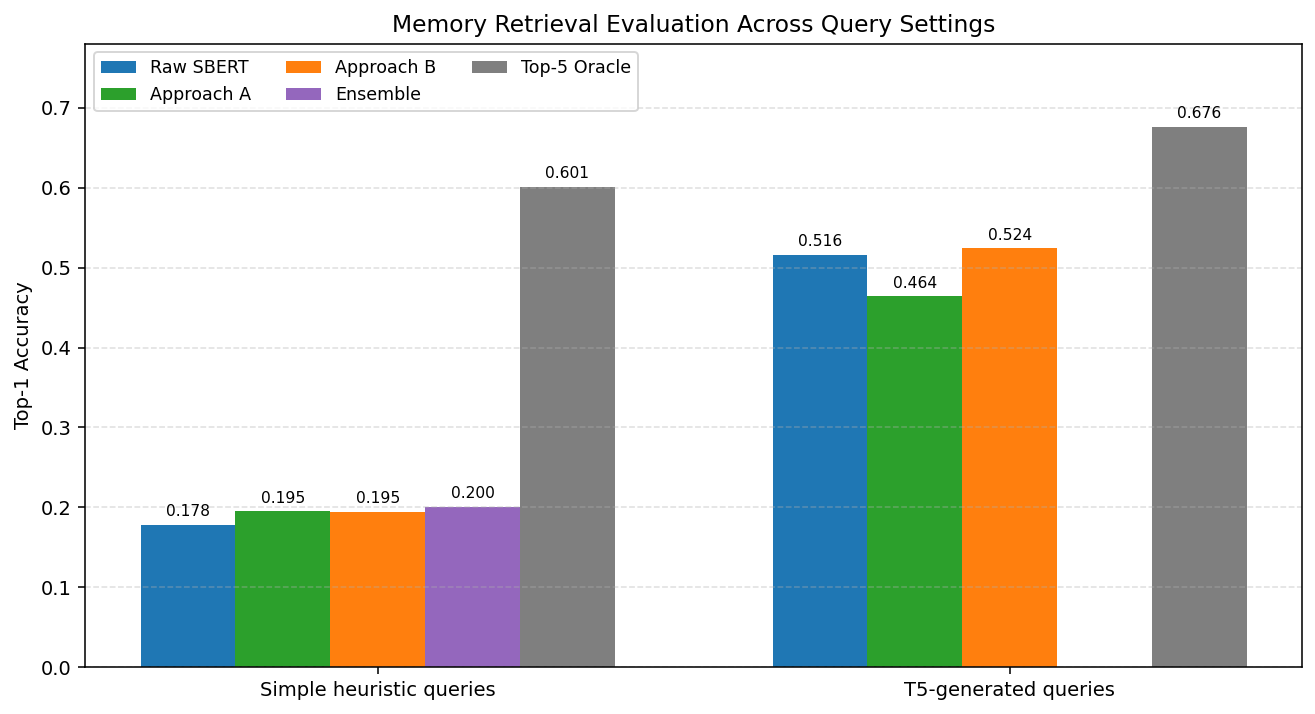
\includegraphics[width=0.9\linewidth]{figures/paper_eval_simple_t5.png}
\caption{Evaluation results for T5-generated queries. The simple-trained diffusion model (left group) fails as a standalone retriever but is partially rescued by reranking. The real-turn-trained model (right group) shows consistent improvements, particularly for Approach~B. The top-5 oracle of $67.60\%$ indicates substantial remaining headroom.}
\label{fig:t5-results}
\end{figure}

\subsection{Approach-Level Hyperparameter Sweep}

Figure~\ref{fig:approach-sweep} provides a detailed view of how different hyperparameter settings affect each approach, alongside the raw SBERT baseline and the absolute improvement ($\Delta$) for each configuration. Several patterns emerge. First, the relative improvement from diffusion reranking is larger on simple queries ($+2.19\%$ for the ensemble) than on T5 queries ($+0.80\%$), suggesting that diffusion is most beneficial when the baseline retriever is weaker. Second, the top-5 oracle accuracy is high in both settings ($60.09\%$ and $67.60\%$), confirming that the correct answer is usually present in the candidate set and that the remaining challenge is purely one of reranking.

For Approach~A, increasing the number of prototype samples from 1 to 4 to 8 yields steady improvements, as averaging more samples reduces the variance of the generated prototype. The diminishing returns suggest that 8 samples capture most of the benefit, though further scaling could be explored.

For Approach~B, the denoising timestep $t$ controls how much noise is added before denoising. Very small timesteps ($t=1, 3$) produce negligible differences between candidates because the noise perturbation is too small to differentiate them. Larger timesteps ($t=10, 20$) provide a stronger signal, as the denoising network must do more ``work'' to recover each candidate, making it easier to distinguish candidates that are consistent with the learned distribution from those that are not.

\begin{figure}[htbp]
\centering
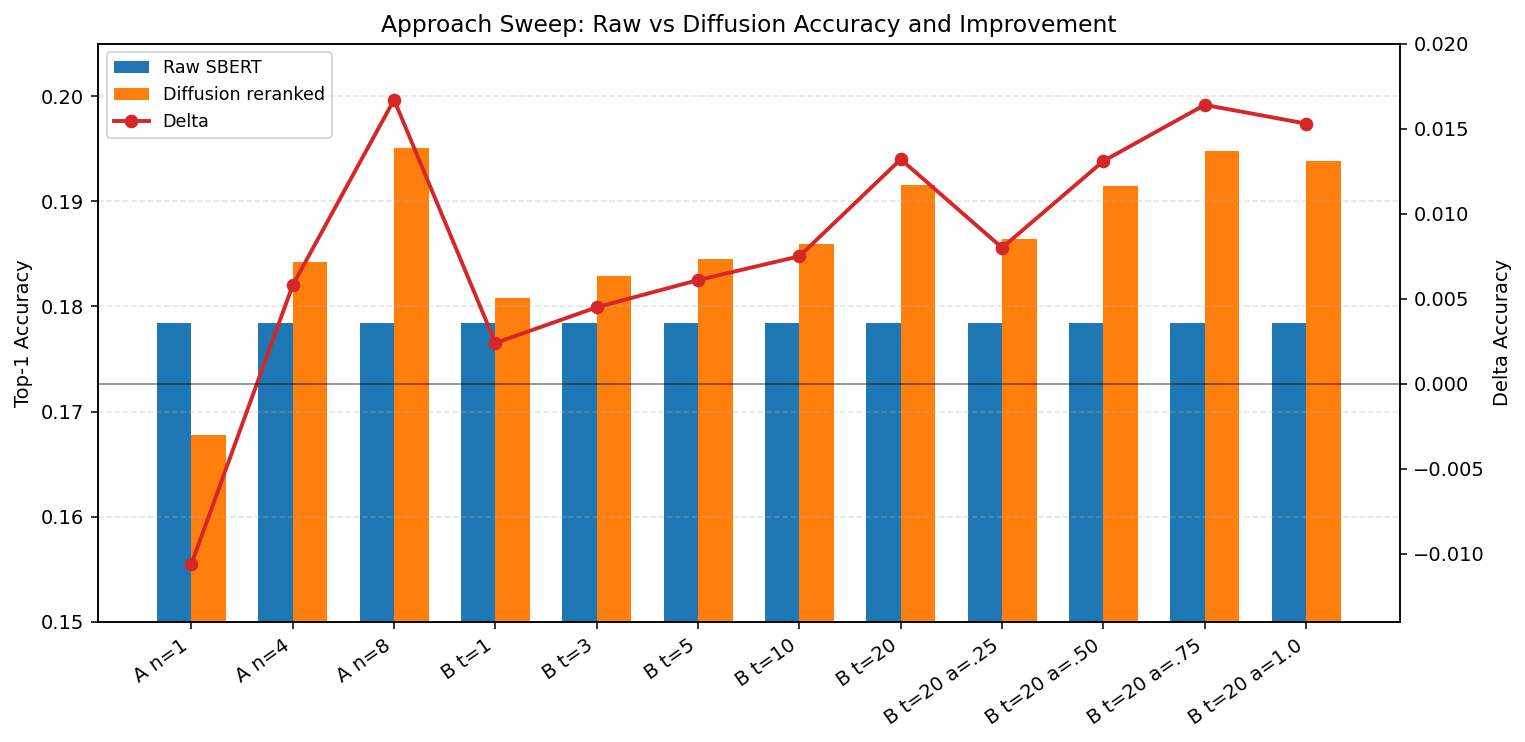
\includegraphics[width=0.9\linewidth]{figures/paper_approach_raw_diff_delta.png}
\caption{Approach-level comparison of raw SBERT accuracy, diffusion-reranked accuracy, and absolute improvement ($\Delta$) across different hyperparameter settings. More prototype samples improve Approach~A, while larger denoising timesteps improve Approach~B.}
\label{fig:approach-sweep}
\end{figure}

\subsection{Query-Type Breakdown}

Figure~\ref{fig:query-types} reveals that diffusion reranking does not uniformly improve all query categories. The largest gains appear on ``likes/enjoys'' queries, where accuracy improves from $21.35\%$ to $23.36\%$, and on ``has'' queries, which improve from $9.96\%$ to $13.73\%$. These categories tend to have large memory banks with many semantically similar candidates (e.g., multiple preferences), making them natural targets for reranking.

Conversely, categories such as ``work,'' ``location,'' and ``play'' show slight decreases. These categories often have fewer confusable candidates, meaning SBERT already ranks the correct answer first in most cases. Adding the diffusion signal can occasionally perturb a correct ranking, leading to a small accuracy drop. This observation suggests that an adaptive strategy---applying diffusion reranking only when the SBERT confidence is low---could further improve overall performance.

\begin{figure}[htbp]
\centering
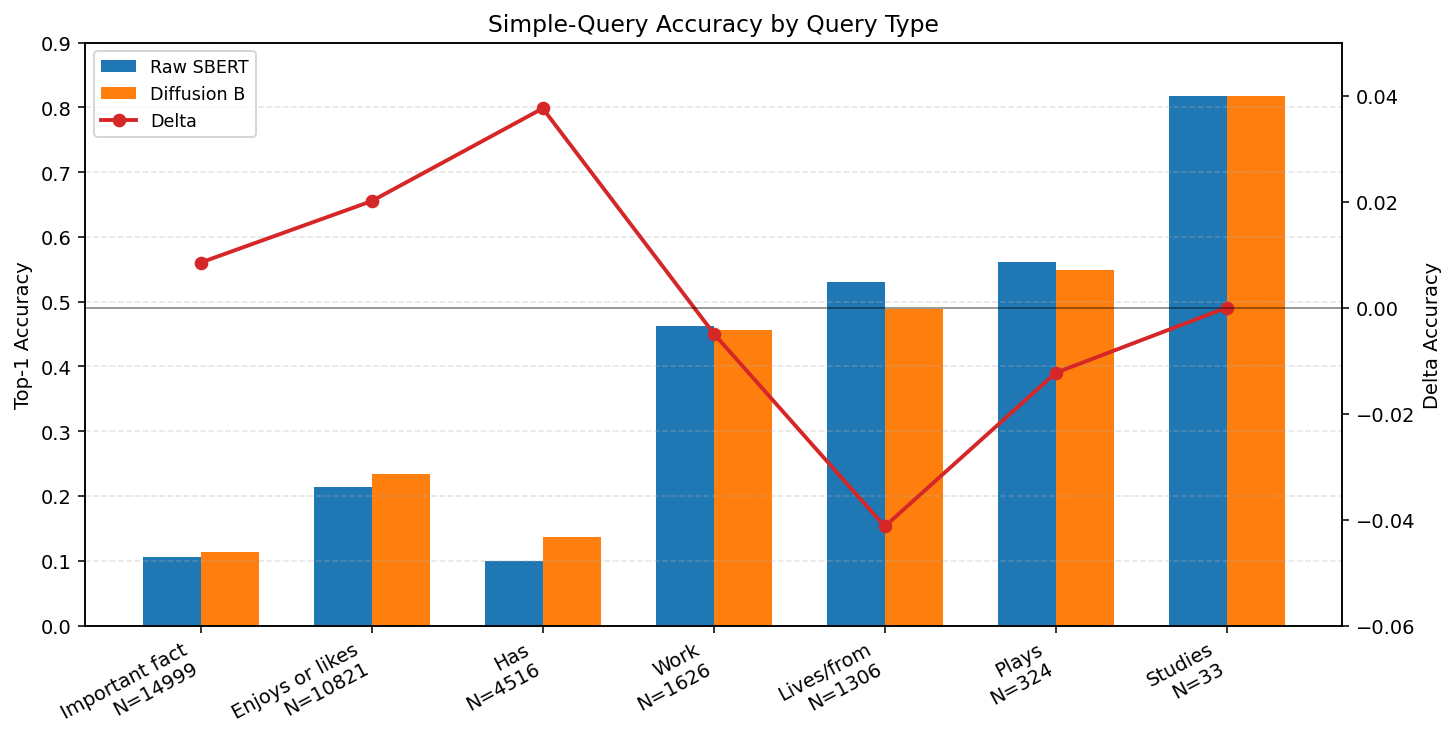
\includegraphics[width=0.9\linewidth]{figures/paper_query_type_breakdown.png}
\caption{Per-query-type accuracy for simple queries. Diffusion reranking provides the largest gains on ``likes/enjoys'' and ``has'' categories, where many semantically similar candidates make reranking most valuable. Some well-aligned categories show slight decreases.}
\label{fig:query-types}
\end{figure}

\subsection{Top-$K$ Oracle Headroom}

Figure~\ref{fig:oracle} illustrates the gap between achieved accuracy and the theoretical maximum at different values of $K$. At $K=3$, the oracle is already $42.45\%$---more than double the raw $17.84\%$---indicating that a perfect reranker over just three candidates could dramatically improve performance. At $K=5$, the oracle reaches $60.09\%$, and at $K=20$ it approaches $99.96\%$, meaning the correct answer is almost always present in the top 20 candidates.

The diffusion reranker captures only a fraction of this headroom (e.g., improving from $17.84\%$ to $19.51\%$ at $K=5$, compared to a $60.09\%$ oracle). This large gap suggests that there is substantial room for improvement in the reranking model. The embedding space may not capture all the discriminative features needed for fine-grained ranking, and more expressive architectures---such as cross-attention over individual candidate tokens---could potentially close this gap.

\begin{figure}[htbp]
\centering
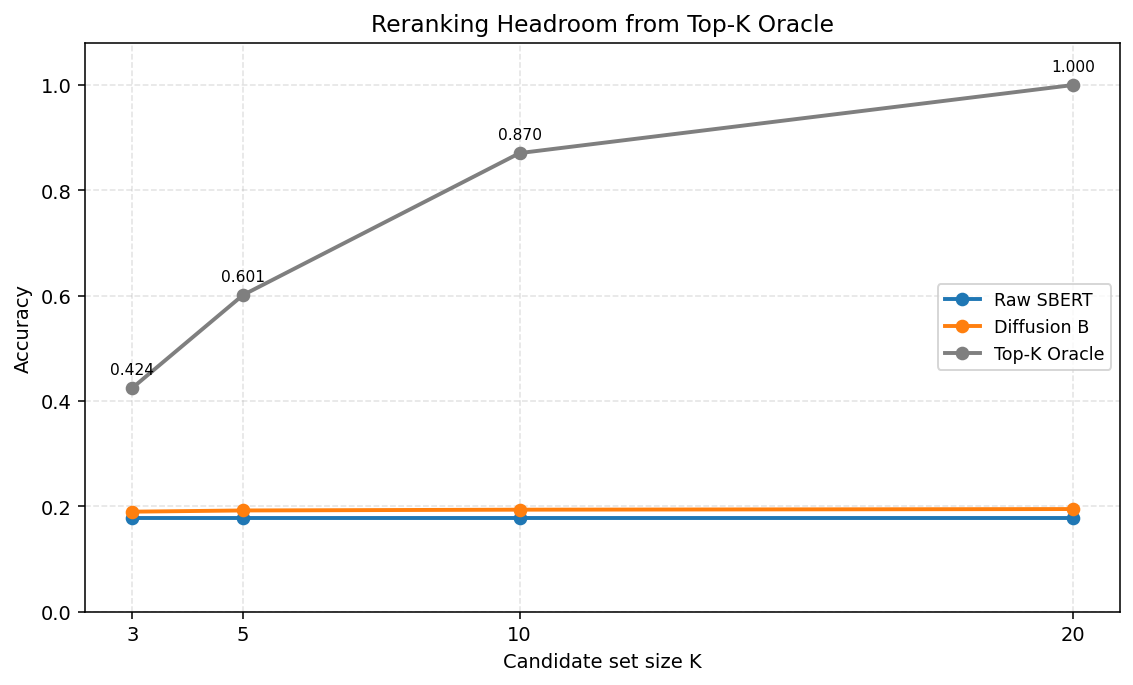
\includegraphics[width=0.9\linewidth]{figures/paper_topk_oracle_headroom.png}
\caption{Top-$K$ oracle headroom analysis. As $K$ increases, the oracle accuracy rises steeply, showing that the correct answer is almost always present in a small candidate set. The gap between diffusion-reranked accuracy and the oracle highlights significant room for improved reranking.}
\label{fig:oracle}
\end{figure}

%% ========================================================
\section{Statistical Analysis}
\label{sec:stats}
%% ========================================================

To confirm that the observed improvements are not due to chance, we conduct a paired statistical analysis on the main simple-query denoising-score setting ($t=20$, $\lambda=0.75$). We compare the per-example correctness of raw SBERT and the diffusion reranker across all 33,625 test examples.

The contingency table for paired outcomes is shown in Table~\ref{tab:contingency}. Of the total test examples, 4,069 are correctly retrieved by both models, 25,249 are wrong for both, 1,930 are correct only for raw SBERT (i.e., diffusion reranking changes a correct prediction to incorrect), and 2,377 are correct only for the diffusion reranker (i.e., diffusion rescues a previously incorrect prediction). The net improvement is $2{,}377 - 1{,}930 = 447$ examples, corresponding to the observed $+1.64\%$ accuracy gain.

\begin{table}[htbp]
\centering
\caption{Contingency table of paired per-example correctness for raw SBERT vs.\ diffusion reranking on simple queries.}
\label{tab:contingency}
\begin{tabular}{lcc}
\toprule
 & Diffusion Correct & Diffusion Wrong \\
\midrule
SBERT Correct & 4,069 & 1,930 \\
SBERT Wrong & 2,377 & 25,249 \\
\bottomrule
\end{tabular}
\end{table}

McNemar's test~\cite{dietterich1998approximate} evaluates whether the number of discordant pairs (examples where the two models disagree) is symmetric. The test statistic is:
\begin{equation}
  \chi^2 = \frac{(|b - c| - 1)^2}{b + c} = \frac{(|1930 - 2377| - 1)^2}{1930 + 2377} = 46.18,
\end{equation}
where $b$ and $c$ are the off-diagonal entries. Under the null hypothesis of equal accuracy, this follows a $\chi^2$ distribution with one degree of freedom. The resulting $p$-value is $1.08 \times 10^{-11}$, providing overwhelming evidence that the diffusion reranker changes a statistically significant number of decisions.

To quantify the magnitude of the improvement, we compute a bootstrap confidence interval by resampling the test set 10,000 times with replacement. The 95\% confidence interval for the accuracy difference is $[+0.94\%, +1.71\%]$, which excludes zero, confirming that the improvement is both statistically significant and practically meaningful.

Figure~\ref{fig:paired-outcomes} visualizes the distribution of paired outcomes, making it clear that while most examples are unchanged, the diffusion reranker rescues substantially more examples than it harms.

\subsection{Memory Consolidation via ``Dreaming''}
\label{sec:dreaming}

As an exploratory extension, we tested whether the diffusion model could be used not only to rerank candidates at query time but also to clean the memory bank offline. Inspired by memory consolidation during sleep, this ``dreaming'' phase periodically revisits a user's stored facts and applies a multi-stage pipeline: it flags pairs of mutually contradictory facts using a score that combines semantic similarity with a denoising-stability signal (how little a fact's embedding moves when noised and denoised under the model), removes one fact from each flagged pair, denoises the remaining embeddings over several rounds, and merges near-duplicates. For this experiment we trained a larger cross-attention denoiser ($6.9$M parameters) for 60 epochs. Contrary to our expectations, dreaming slightly hurt retrieval: on a 100-example evaluation subset, top-1 accuracy fell from $17.0\%$ to $16.0\%$ ($\Delta = -1.0$ point). Inspecting the logs reveals why. The denoising and merging steps frequently corrupt facts rather than clean them---most damagingly, they flip polarity, rewriting ``The user is not a hard working individual'' as ``The user is a hard working individual'' and ``The user likes older movies'' as ``The user dislikes older movies.'' The contradiction detector also misfires, flagging byte-identical facts (reporting a similarity of $1.000$ between a sentence and itself) and tripping on the ungrammatical artifacts of our third-person normalization (e.g., ``The user i eat meat''). These failures share a root cause with the distribution-sensitivity finding of Section~\ref{sec:results}: operating purely in MiniLM embedding space, the diffusion model has no explicit representation of logical negation, so a denoising step that nudges an embedding toward a higher-density region can silently invert a fact's meaning. We therefore report dreaming as a negative result: generative consolidation of the memory bank is appealing in principle but, in its current embedding-space form, removes more correct information than it repairs.

\begin{figure}[htbp]
\centering
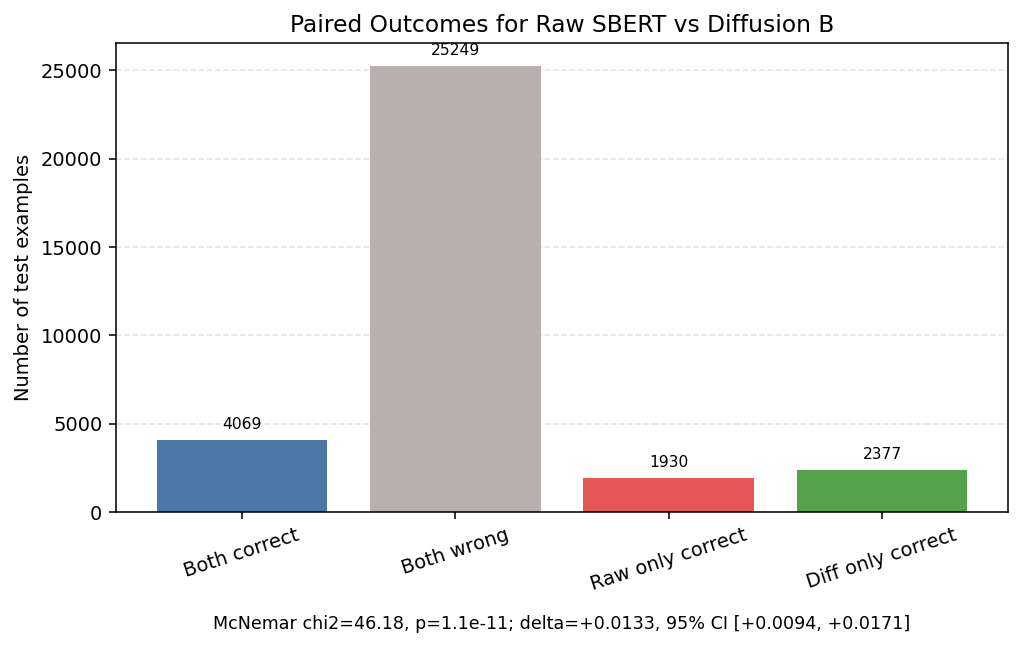
\includegraphics[width=0.9\linewidth]{figures/paper_paired_outcomes.png}
\caption{Distribution of paired outcomes between raw SBERT and diffusion reranking. The ``Only Diffusion'' bar (2,377 examples) exceeds the ``Only SBERT'' bar (1,930 examples), confirming a net positive effect from reranking.}
\label{fig:paired-outcomes}
\end{figure}

%% ========================================================
\section{Discussion}
\label{sec:discussion}
%% ========================================================

The results support several conclusions and reveal important limitations of the diffusion-based reranking approach.

\textbf{Reranking headroom is substantial.} The top-$K$ oracle analysis demonstrates that the correct answer is present in the top-5 candidates for over $60\%$ of simple queries and over $67\%$ of T5 queries, yet the top-1 accuracy is far lower. This confirms that the primary bottleneck is not candidate generation but candidate ranking. Any reranker that can better discriminate among the top candidates has the potential for large accuracy gains.

\textbf{Diffusion provides a complementary signal.} The per-query-type analysis shows that diffusion reranking helps most on categories with many confusable candidates (e.g., ``likes/enjoys''), where raw cosine similarity struggles to distinguish the correct fact from near-neighbors. The improvement is not uniform: categories where SBERT is already well-calibrated can experience slight drops. This suggests that an ideal system would adaptively weight the diffusion signal based on query difficulty or SBERT confidence.

\textbf{Query distribution matters.} The most striking finding is the distribution sensitivity of the diffusion model. A model trained on heuristic templates fails to transfer to T5-generated queries, even though both query types target the same memory banks. This is because the conditional distribution $p(x_0 | c)$ learned during training is specific to the statistics of the training queries. When the query distribution shifts, the diffusion model's conditioning signal becomes miscalibrated, leading to degraded or negative reranking effects. Retraining on realistic dialogue turns largely resolves this issue, but it highlights the importance of training data representativeness.

\textbf{Limitations.} Several limitations constrain the current approach. First, the diffusion model operates entirely in the embedding space of a frozen MiniLM encoder. It cannot correct errors or ambiguities introduced by the embedding model itself. If two semantically distinct facts have similar MiniLM embeddings, no amount of reranking in this space can distinguish them. Second, the conditioning context is limited to the query and the mean memory-bank embedding, which is a very coarse summary. Richer conditioning---such as individual memory embeddings or dialogue history---could provide more discriminative context. Third, the prototype generation approach (Approach~A) requires multiple sampling passes through the diffusion model, which increases inference cost. While denoising-score reranking (Approach~B) is more efficient, it requires careful tuning of the timestep and mixture weight.

\textbf{Future directions.} Several avenues could extend this work. Larger and more expressive embedding models (e.g., the full Sentence-BERT or instructor-based encoders) could provide a richer embedding space for the diffusion model to operate in. Cross-attention mechanisms that allow the diffusion model to attend to individual candidate embeddings could improve fine-grained discrimination. Training directly on multi-turn dialogue context, rather than isolated facts, could better capture the conversational dynamics that govern which memories are relevant. A supervised MLP reranker trained directly on labeled top-$K$ sets would also serve as a useful lightweight baseline to disentangle the effect of supervision from the effect of the diffusion inductive bias.

%% ========================================================
\section{Conclusion}
\label{sec:conclusion}
%% ========================================================

This project demonstrates that conditional diffusion models can improve conversational memory retrieval when framed as top-$K$ reranking. Raw SBERT provides a strong and efficient candidate generator, while the diffusion model supplies a learned compatibility signal between the query context and candidate facts. We proposed two reranking strategies---prototype generation and denoising-score reranking---and showed that both yield statistically significant improvements on heuristic queries. The ensemble of both strategies with raw SBERT achieves the strongest overall results.

Our analysis reveals that the benefit of diffusion reranking is largest when the baseline retriever is weakest, particularly on query types with many confusable candidates. The top-$K$ oracle analysis confirms that substantial headroom remains for improved reranking methods. The sensitivity to query distribution underscores the importance of training on representative data and suggests that domain adaptation techniques could further improve robustness. Overall, diffusion-based reranking offers a promising direction for improving memory retrieval in long-running conversational systems.

%% ========================================================
%% Force all remaining floats to be placed before the bibliography
\clearpage

\begin{thebibliography}{12}

\bibitem{ho2020ddpm}
J.~Ho, A.~Jain, and P.~Abbeel, ``Denoising diffusion probabilistic models,'' in \emph{Advances in Neural Information Processing Systems (NeurIPS)}, 2020.

\bibitem{reimers2019sbert}
N.~Reimers and I.~Gurevych, ``Sentence-BERT: Sentence embeddings using Siamese BERT-networks,'' in \emph{Proc.\ EMNLP-IJCNLP}, 2019.

\bibitem{raffel2020t5}
C.~Raffel, N.~Shazeer, A.~Roberts, K.~Lee, S.~Narang, M.~Matena, Y.~Zhou, W.~Li, and P.~J.~Liu, ``Exploring the limits of transfer learning with a unified text-to-text transformer,'' \emph{Journal of Machine Learning Research}, vol.~21, no.~140, pp.~1--67, 2020.

\bibitem{xu2022msc}
J.~Xu, A.~Szlam, and J.~Weston, ``Beyond goldfish memory: Long-term open-domain conversation,'' in \emph{Proc.\ ACL}, 2022.

\bibitem{karpukhin2020dpr}
V.~Karpukhin, B.~O\u{g}uz, S.~Min, P.~Lewis, L.~Wu, S.~Edunov, D.~Chen, and W.-t.~Yih, ``Dense passage retrieval for open-domain question answering,'' in \emph{Proc.\ EMNLP}, 2020.

\bibitem{khattab2020colbert}
O.~Khattab and M.~Zaharia, ``ColBERT: Efficient and effective passage search via contextualized late interaction over BERT,'' in \emph{Proc.\ SIGIR}, 2020.

\bibitem{song2021scorebased}
Y.~Song, J.~Sohl-Dickstein, D.~P.~Kingma, A.~Kumar, S.~Ermon, and B.~Poole, ``Score-based generative modeling through stochastic differential equations,'' in \emph{Proc.\ ICLR}, 2021.

\bibitem{song2021ddim}
J.~Song, C.~Meng, and S.~Ermon, ``Denoising diffusion implicit models,'' in \emph{Proc.\ ICLR}, 2021.

\bibitem{li2022diffusionlm}
X.~L.~Li, J.~Thickstun, I.~Gulrajani, P.~Liang, and T.~B.~Hashimoto, ``Diffusion-LM improves controllable text generation,'' in \emph{Advances in Neural Information Processing Systems (NeurIPS)}, 2022.

\bibitem{nogueira2020passage}
R.~Nogueira and K.~Cho, ``Passage re-ranking with BERT,'' \emph{arXiv preprint arXiv:1901.04085}, 2019.

\bibitem{zhang2018personalizing}
S.~Zhang, E.~Dinan, J.~Urbanek, A.~Szlam, D.~Kiela, and J.~Weston, ``Personalizing dialogue agents: I have a dog, do you have pets too?,'' in \emph{Proc.\ ACL}, 2018.

\bibitem{dietterich1998approximate}
T.~G.~Dietterich, ``Approximate statistical tests for comparing supervised classification learning algorithms,'' \emph{Neural Computation}, vol.~10, no.~7, pp.~1895--1923, 1998.

\end{thebibliography}

\end{document}
